% This is a Basic Assignment Paper but with like Code and stuff allowed in it. 

\documentclass[11pt]{article}

% Preamble

\usepackage[margin=1in]{geometry}
\usepackage{amsfonts, amsmath, amssymb}
\usepackage{fancyhdr, float, graphicx}
\usepackage[utf8]{inputenc} % Required for inputting international characters
\usepackage[T1]{fontenc} % Output font encoding for international characters
\usepackage{fouriernc} % Use the New Century Schoolbook font
\usepackage[nottoc, notlot, notlof]{tocbibind}
\usepackage{listings}
\usepackage{xcolor}
\usepackage{karnaugh-map}
\usepackage{pdfpages}

\definecolor{codegreen}{rgb}{0,0.6,0}
\definecolor{codegray}{rgb}{0.5,0.5,0.5}
\definecolor{codepurple}{rgb}{0.58,0,0.82}
\definecolor{backcolour}{rgb}{0.95,0.95,0.92}

\lstdefinestyle{mystyle}{
    backgroundcolor=\color{backcolour},   
    commentstyle=\color{codegreen},
    keywordstyle=\color{magenta},
    numberstyle=\tiny\color{codegray},
    stringstyle=\color{codepurple},
    basicstyle=\ttfamily\footnotesize,
    breakatwhitespace=false,         
    breaklines=true,                 
    captionpos=b,                    
    keepspaces=true,                 
    numbers=left,                    
    numbersep=5pt,                  
    showspaces=false,                
    showstringspaces=false,
    showtabs=false,                  
    tabsize=2
}

\lstset{style=mystyle}

% Header and Footer
\pagestyle{fancy}
\fancyhead{}
\fancyfoot{}
\fancyhead[L]{\textit{\Large{DECA Assignment 1}}}
%\fancyhead[R]{\textit{something}}
\fancyfoot[C]{\thepage}
\renewcommand{\footrulewidth}{1pt}



% Other Doc Editing
% \parindent 0ex
%\renewcommand{\baselinestretch}{1.5}

\begin{document}

\begin{titlepage}
	\centering

	%---------------------------NAMES-------------------------------

	\huge\textsc{
		MIT World Peace University
	}\\

	\vspace{0.75\baselineskip} % space after Uni Name

	\LARGE{
		Digital Electronics and Computer Architecture\\
		Second Year B. Tech, Semester 3
	}

	\vfill % space after Sub Name

	%--------------------------TITLE-------------------------------

	\rule{\textwidth}{1.6pt}\vspace*{-\baselineskip}\vspace*{2pt}
	\rule{\textwidth}{0.6pt}
	\vspace{0.75\baselineskip} % Whitespace above the title



	\huge{\textsc{
			4 Bit Code Conversion between Binary and Gray Code using Basic Logic Gates
		}} \\



	\vspace{0.5\baselineskip} % Whitespace below the title
	\rule{\textwidth}{0.6pt}\vspace*{-\baselineskip}\vspace*{2.8pt}
	\rule{\textwidth}{1.6pt}

	\vspace{1\baselineskip} % Whitespace after the title block

	%--------------------------SUBTITLE --------------------------	

	\LARGE\textsc{
		Practical Report
	} % Subtitle or further description
	\vfill

	%--------------------------AUTHOR-------------------------------

	Prepared By
	\vspace{0.5\baselineskip} % Whitespace before the editors

	\Large{
		Krishnaraj Thadesar \\
		Cyber Security and Forensics\\
		Batch A2, PA 34
	}


	\vspace{0.5\baselineskip} % Whitespace below the editor list
	\today

\end{titlepage}


\tableofcontents
\thispagestyle{empty}
\clearpage


\setcounter{page}{1}

\section{Problem Statement}
Design and Implementation of 4 Bit code convertors using Basic Logic Gates.

\begin{enumerate}
	\item 4 Bit Binary to Gray Code
	\item 4 Bit Gray to Binary Code
\end{enumerate}

\section{ICs Used}
74LS86 (Quad 2-Input Exclusive - OR Gates)

\section{Platform Used}
Digital Trainer Kit

\section{Theory}

\subsection{Involved Truth Tables}

\subsubsection{Binary to Gray Code}

\begin{table}[H]
	\begin{tabular}{|llll||llll|}
		\hline
		\multicolumn{4}{|l|}{\textbf{Binary Code}} & \multicolumn{4}{l|}{\textbf{Gray Code}}                                                                                                                                     \\ \hline
		\multicolumn{1}{|l|}{$B_3$}                & \multicolumn{1}{l|}{$B_2$}              & \multicolumn{1}{l|}{$B_1$} & $B_0$ & \multicolumn{1}{l|}{$G_3$} & \multicolumn{1}{l|}{$G_2$} & \multicolumn{1}{l|}{$G_1$} & $G_0$ \\ \hline
		\multicolumn{1}{|l|}{0}                    & \multicolumn{1}{l|}{0}                  & \multicolumn{1}{l|}{0}     & 0     & \multicolumn{1}{l|}{0}     & \multicolumn{1}{l|}{0}     & \multicolumn{1}{l|}{0}     & 0     \\ \hline
		\multicolumn{1}{|l|}{0}                    & \multicolumn{1}{l|}{0}                  & \multicolumn{1}{l|}{0}     & 1     & \multicolumn{1}{l|}{0}     & \multicolumn{1}{l|}{0}     & \multicolumn{1}{l|}{0}     & 1     \\ \hline
		\multicolumn{1}{|l|}{0}                    & \multicolumn{1}{l|}{0}                  & \multicolumn{1}{l|}{1}     & 0     & \multicolumn{1}{l|}{0}     & \multicolumn{1}{l|}{0}     & \multicolumn{1}{l|}{1}     & 1     \\ \hline
		\multicolumn{1}{|l|}{0}                    & \multicolumn{1}{l|}{0}                  & \multicolumn{1}{l|}{1}     & 1     & \multicolumn{1}{l|}{0}     & \multicolumn{1}{l|}{0}     & \multicolumn{1}{l|}{1}     & 0     \\ \hline
		\multicolumn{1}{|l|}{0}                    & \multicolumn{1}{l|}{1}                  & \multicolumn{1}{l|}{0}     & 0     & \multicolumn{1}{l|}{0}     & \multicolumn{1}{l|}{1}     & \multicolumn{1}{l|}{1}     & 0     \\ \hline
		\multicolumn{1}{|l|}{0}                    & \multicolumn{1}{l|}{1}                  & \multicolumn{1}{l|}{0}     & 1     & \multicolumn{1}{l|}{0}     & \multicolumn{1}{l|}{1}     & \multicolumn{1}{l|}{1}     & 1     \\ \hline
		\multicolumn{1}{|l|}{0}                    & \multicolumn{1}{l|}{1}                  & \multicolumn{1}{l|}{1}     & 0     & \multicolumn{1}{l|}{0}     & \multicolumn{1}{l|}{1}     & \multicolumn{1}{l|}{0}     & 1     \\ \hline
		\multicolumn{1}{|l|}{0}                    & \multicolumn{1}{l|}{1}                  & \multicolumn{1}{l|}{1}     & 1     & \multicolumn{1}{l|}{0}     & \multicolumn{1}{l|}{1}     & \multicolumn{1}{l|}{0}     & 0     \\ \hline
		\multicolumn{1}{|l|}{1}                    & \multicolumn{1}{l|}{0}                  & \multicolumn{1}{l|}{0}     & 0     & \multicolumn{1}{l|}{1}     & \multicolumn{1}{l|}{1}     & \multicolumn{1}{l|}{0}     & 0     \\ \hline
		\multicolumn{1}{|l|}{1}                    & \multicolumn{1}{l|}{0}                  & \multicolumn{1}{l|}{0}     & 1     & \multicolumn{1}{l|}{1}     & \multicolumn{1}{l|}{1}     & \multicolumn{1}{l|}{0}     & 1     \\ \hline
		\multicolumn{1}{|l|}{1}                    & \multicolumn{1}{l|}{0}                  & \multicolumn{1}{l|}{1}     & 0     & \multicolumn{1}{l|}{1}     & \multicolumn{1}{l|}{1}     & \multicolumn{1}{l|}{1}     & 1     \\ \hline
		\multicolumn{1}{|l|}{1}                    & \multicolumn{1}{l|}{0}                  & \multicolumn{1}{l|}{1}     & 1     & \multicolumn{1}{l|}{1}     & \multicolumn{1}{l|}{1}     & \multicolumn{1}{l|}{1}     & 0     \\ \hline
		\multicolumn{1}{|l|}{1}                    & \multicolumn{1}{l|}{1}                  & \multicolumn{1}{l|}{0}     & 0     & \multicolumn{1}{l|}{1}     & \multicolumn{1}{l|}{0}     & \multicolumn{1}{l|}{1}     & 0     \\ \hline
		\multicolumn{1}{|l|}{1}                    & \multicolumn{1}{l|}{1}                  & \multicolumn{1}{l|}{0}     & 1     & \multicolumn{1}{l|}{1}     & \multicolumn{1}{l|}{0}     & \multicolumn{1}{l|}{1}     & 1     \\ \hline
		\multicolumn{1}{|l|}{1}                    & \multicolumn{1}{l|}{1}                  & \multicolumn{1}{l|}{1}     & 0     & \multicolumn{1}{l|}{1}     & \multicolumn{1}{l|}{0}     & \multicolumn{1}{l|}{0}     & 1     \\ \hline
		\multicolumn{1}{|l|}{1}                    & \multicolumn{1}{l|}{1}                  & \multicolumn{1}{l|}{1}     & 1     & \multicolumn{1}{l|}{1}     & \multicolumn{1}{l|}{0}     & \multicolumn{1}{l|}{0}     & 0     \\ \hline
	\end{tabular}
\end{table}

\subsubsection{Gray to Binary Code}
\begin{table}[H]
	\begin{tabular}{|llll||llll|}
		\hline
		\multicolumn{4}{|l|}{\textbf{Gray Code}} & \multicolumn{4}{l|}{\textbf{Binary Code}}
		\\ \hline
		\multicolumn{1}{|l|}{$G_3$}              & \multicolumn{1}{l|}{$G_2$}                & \multicolumn{1}{l|}{$G_1$} & $G_0$ & \multicolumn{1}{l|}{$B_3$} & \multicolumn{1}{l|}{$B_2$} & \multicolumn{1}{l|}{$B_1$} & $B_0$ \\ \hline
		\multicolumn{1}{|l|}{0}                  & \multicolumn{1}{l|}{0}                    & \multicolumn{1}{l|}{0}     & 0     & \multicolumn{1}{l|}{0}     & \multicolumn{1}{l|}{0}     & \multicolumn{1}{l|}{0}     & 0     \\ \hline
		\multicolumn{1}{|l|}{0}                  & \multicolumn{1}{l|}{0}                    & \multicolumn{1}{l|}{0}     & 1     & \multicolumn{1}{l|}{0}     & \multicolumn{1}{l|}{0}     & \multicolumn{1}{l|}{0}     & 1     \\ \hline
		\multicolumn{1}{|l|}{0}                  & \multicolumn{1}{l|}{0}                    & \multicolumn{1}{l|}{1}     & 0     & \multicolumn{1}{l|}{0}     & \multicolumn{1}{l|}{0}     & \multicolumn{1}{l|}{1}     & 1     \\ \hline
		\multicolumn{1}{|l|}{0}                  & \multicolumn{1}{l|}{0}                    & \multicolumn{1}{l|}{1}     & 1     & \multicolumn{1}{l|}{0}     & \multicolumn{1}{l|}{0}     & \multicolumn{1}{l|}{1}     & 0     \\ \hline
		\multicolumn{1}{|l|}{0}                  & \multicolumn{1}{l|}{1}                    & \multicolumn{1}{l|}{0}     & 0     & \multicolumn{1}{l|}{0}     & \multicolumn{1}{l|}{1}     & \multicolumn{1}{l|}{1}     & 1     \\ \hline
		\multicolumn{1}{|l|}{0}                  & \multicolumn{1}{l|}{1}                    & \multicolumn{1}{l|}{0}     & 1     & \multicolumn{1}{l|}{0}     & \multicolumn{1}{l|}{1}     & \multicolumn{1}{l|}{1}     & 0     \\ \hline
		\multicolumn{1}{|l|}{0}                  & \multicolumn{1}{l|}{1}                    & \multicolumn{1}{l|}{1}     & 0     & \multicolumn{1}{l|}{0}     & \multicolumn{1}{l|}{1}     & \multicolumn{1}{l|}{0}     & 0     \\ \hline
		\multicolumn{1}{|l|}{0}                  & \multicolumn{1}{l|}{1}                    & \multicolumn{1}{l|}{1}     & 1     & \multicolumn{1}{l|}{0}     & \multicolumn{1}{l|}{1}     & \multicolumn{1}{l|}{0}     & 1     \\ \hline
		\multicolumn{1}{|l|}{1}                  & \multicolumn{1}{l|}{1}                    & \multicolumn{1}{l|}{0}     & 0     & \multicolumn{1}{l|}{1}     & \multicolumn{1}{l|}{0}     & \multicolumn{1}{l|}{0}     & 0     \\ \hline
		\multicolumn{1}{|l|}{1}                  & \multicolumn{1}{l|}{1}                    & \multicolumn{1}{l|}{0}     & 1     & \multicolumn{1}{l|}{1}     & \multicolumn{1}{l|}{0}     & \multicolumn{1}{l|}{0}     & 1     \\ \hline
		\multicolumn{1}{|l|}{1}                  & \multicolumn{1}{l|}{1}                    & \multicolumn{1}{l|}{1}     & 0     & \multicolumn{1}{l|}{1}     & \multicolumn{1}{l|}{0}     & \multicolumn{1}{l|}{1}     & 1     \\ \hline
		\multicolumn{1}{|l|}{1}                  & \multicolumn{1}{l|}{1}                    & \multicolumn{1}{l|}{1}     & 1     & \multicolumn{1}{l|}{1}     & \multicolumn{1}{l|}{0}     & \multicolumn{1}{l|}{1}     & 0     \\ \hline
		\multicolumn{1}{|l|}{1}                  & \multicolumn{1}{l|}{0}                    & \multicolumn{1}{l|}{0}     & 0     & \multicolumn{1}{l|}{1}     & \multicolumn{1}{l|}{1}     & \multicolumn{1}{l|}{1}     & 1     \\ \hline
		\multicolumn{1}{|l|}{1}                  & \multicolumn{1}{l|}{0}                    & \multicolumn{1}{l|}{0}     & 1     & \multicolumn{1}{l|}{1}     & \multicolumn{1}{l|}{1}     & \multicolumn{1}{l|}{1}     & 0     \\ \hline
		\multicolumn{1}{|l|}{1}                  & \multicolumn{1}{l|}{0}                    & \multicolumn{1}{l|}{1}     & 0     & \multicolumn{1}{l|}{1}     & \multicolumn{1}{l|}{1}     & \multicolumn{1}{l|}{0}     & 0     \\ \hline
		\multicolumn{1}{|l|}{1}                  & \multicolumn{1}{l|}{0}                    & \multicolumn{1}{l|}{1}     & 1     & \multicolumn{1}{l|}{1}     & \multicolumn{1}{l|}{1}     & \multicolumn{1}{l|}{0}     & 1     \\ \hline
	\end{tabular}
\end{table}

\subsubsection{XOR Gate}
\begin{table}[H]
	\begin{tabular}{|l|l|l|}
		\hline
		\textbf{A} & \textbf{B} & \textbf{Y} \\ \hline
		0          & 0          & 0          \\ \hline
		0          & 1          & 1          \\ \hline
		1          & 0          & 1          \\ \hline
		1          & 1          & 0          \\ \hline
	\end{tabular}
\end{table}

\pagebreak

\subsection{Reduced Boolean Expressions from Respective Karnaugh Maps}

\subsubsection{Karnaugh Maps for Binary to Gray}


\textbf{1. For Variable $G_3$}\\

\begin{karnaugh-map}[4][4][1][$B_0$][$B_1$][$B_2$][$B_3$]
\minterms{12, 13, 14, 15, 8, 9, 10, 11}
% \autoterms[0]
\implicant{12}{10}
\end{karnaugh-map}

\noindent
\textit{Simplification of Karnaugh Map Expression from the above K - Map : }

\begin{eqnarray}
	G_3 = B_3
\end{eqnarray}



\noindent
\textbf{1. For Variable $G_2$}\\

\begin{karnaugh-map}[4][4][1][$B_0$][$B_1$][$B_2$][$B_3$]
\minterms{4, 5, 6, 7, 8, 9, 10, 11}
% \autoterms[0]
\implicant{4}{6}
\implicant{8}{10}
\end{karnaugh-map}

\noindent
\textit{Simplification of Karnaugh Map Expression from the above K - Map : }

\begin{eqnarray}
	G_2 = \overline{B_3}B_2 + \overline{B_2}B_3 \\
	G_2 = B_3 \oplus B_2
\end{eqnarray}



\noindent
\textbf{1. For Variable $G_1$}\\

\begin{karnaugh-map}[4][4][1][$B_0$][$B_1$][$B_2$][$B_3$]
\minterms{2, 3, 4, 5, 10, 11, 12, 13}
% \autoterms[0]
\implicant{4}{13}
\implicantedge{3}{2}{11}{10}
\end{karnaugh-map}

\noindent
\textit{Simplification of Karnaugh Map Expression from the above K - Map : }

\begin{eqnarray}
	G_1 = \overline{B_1}B_2 + \overline{B_2}B_1 \\
	G_1 = B_2 \oplus B_1
\end{eqnarray}



\noindent
\textbf{1. For Variable $G_0$}\\

\begin{karnaugh-map}[4][4][1][$B_0$][$B_1$][$B_2$][$B_3$]
\minterms{1, 2, 5, 6, 9, 10, 13, 14}
% \autoterms[0]
\implicant{1}{9}
\implicant{2}{10}
\end{karnaugh-map}

\noindent
\textit{Simplification of Karnaugh Map Expression from the above K - Map : }

\begin{eqnarray}
	G_0 = \overline{B_0}B_1 + \overline{B_1}B_0 \\
	G_0 = B_1 \oplus B_0
\end{eqnarray}


\pagebreak



\noindent
\textbf{Final Expressions for Binary to Gray}
\begin{eqnarray}
	G_0 = B_3\\
	G_2 = B_3 \oplus B_2 \\
	G_1 = B_2 \oplus B_1 \\
	G_0 = B_1 \oplus B_0
\end{eqnarray}

\subsubsection{Karnaugh Maps for Gray to Binary}
There is difference when we plot minterms for K maps here, as K Maps are inherently written in Gray code, when we write the min terms, we have to fill them in the respective Gray code > Decimal value, instead of the usual binary > Decimal value.

\noindent
\textbf{1. For Variable $B_3$}\\

\begin{karnaugh-map}[4][4][1][$G_0$][$G_1$][$G_2$][$G_3$]
\minterms{12, 13, 14, 15, 8, 9, 10, 11}
% \autoterms[0]
\implicant{12}{10}
\end{karnaugh-map}
\noindent

\textit{Simplification of Karnaugh Map Expression from the above K - Map : }

\begin{eqnarray}
	B_3 = G_3
\end{eqnarray}


\noindent
\textbf{1. For Variable $B_2$}\\

\begin{karnaugh-map}[4][4][1][$G_0$][$G_1$][$G_2$][$G_3$]
\minterms{4, 5, 6, 7, 8, 9, 10, 11}
% \autoterms[0]
\implicant{4}{6}
\implicant{8}{10}
\end{karnaugh-map}
\noindent

\textit{Simplification of Karnaugh Map Expression from the above K - Map : }



\begin{equation}
	B_2 = \overline{G_2}G_3 + \overline{G_2}G_2
	B_2 = G_3 \oplus G_2
\end{equation}

\noindent
\textbf{1. For Variable $B_1$}\\

\begin{karnaugh-map}[4][4][1][$G_0$][$G_1$][$G_2$][$G_3$]
\minterms{2, 3, 4, 5, 8, 9, 14, 15}
% \autoterms[0]
\implicant{3}{2}
\implicant{4}{5}
\implicant{8}{9}
\implicant{15}{14}
\end{karnaugh-map}
\noindent

\textit{Simplification of Karnaugh Map Expression from the above K - Map : }

\begin{equation}
	\begin{gathered}
		B_1=\bar{G_3} G_2 \bar{G_1}+G_3 \bar{G_2} \bar{G_1}+\bar{G_3} \bar{G_2} G_1+G_3 G_2 G_1 \\
		=G_3(\bar{G_2} \bar{G_1}+G_2 G_1)+\bar{G_3}(G_2 \bar{G_1}+\bar{G_2} G_1) \\
		\quad=G_3(\overline{G_2 \bar{G_1}}+\bar{G_2} G_1)+\bar{G_3}(G_2 \bar{G_1}+\bar{G_2} G_1) \\
		=G_3(\overline{G_2 \oplus G_1})+\bar{G_3}(\overline{G_2 \oplus G_1})=G_3 \oplus G_2 \oplus G_1
	\end{gathered}
\end{equation}


\begin{eqnarray}
	B_1 = G_3 \oplus G_2 \oplus G_1
\end{eqnarray}

\noindent
\textbf{1. For Variable $B_0$}\\

\begin{karnaugh-map}[4][4][1][$G_0$][$G_1$][$G_2$][$G_3$]
\minterms{1, 2, 4, 7, 8, 11, 13, 14}
% \autoterms[0]
\implicant{1}{1}
\implicant{2}{2}
\implicant{4}{4}
\implicant{7}{7}
\implicant{8}{8}
\implicant{11}{11}
\implicant{13}{13}
\implicant{14}{14}
\end{karnaugh-map}

\noindent
\textit{Simplification of Karnaugh Map Expression from the above K - Map : }
\begin{equation}
	\begin{gathered}
		B_0=\bar{G_3} \bar{G_2} \bar{G_0} G_0+\bar{G_3} \bar{G_2} G_1 \bar{G_0}+\bar{G_3} G_2 \bar{G_1} \bar{G_0}+\bar{G_3} G_2 G_1 G_0+G_3 G_2 \bar{G_1} G_0+G_3 G_2 G_1 \bar{G_0}+G_3 \bar{G_2} \bar{G_1} \bar{G_0} \\
		+G_3 \bar{G_2} G_1 G_0=G_3 \oplus G_2 \oplus G_1 \oplus G_0
	\end{gathered}
	\end{equation}
\begin{eqnarray}
	B_0 = G_3 \oplus G_2 \oplus G_1 \oplus + G_0
\end{eqnarray}


\noindent
\textbf{Final Expressions for Gray to Binary}
\begin{eqnarray}
	B_3 = G_3 \\
	B_2 = G_3 \oplus G_2 \\
	B_1 = G_3 \oplus G_2 \oplus G_1\\
	B_0 = G_3 \oplus G_2 \oplus G_1 \oplus + G_0
\end{eqnarray}

\section{Design and Implementation}
% here we can draw the logic gate design diagram thing for both binary to gray and gray to binary 

\begin{enumerate}
	\item We only need XOR gates for this so, we can just start with drawing the Inputs for Binary to Gray B0, B1, B2, B3 and Gray to Binary G0, G1, G2, G3 respectively. 
	\item Refer to the final Expressions obtained from the K-Maps for each conversion. 
	\item Join the inputs to the respective Gate Inputs
	\item To make the Circuit Diagram, Replace the Gates with their respective ICs, in this case IC7486 for XOR gates, and join inputs of the IC to the Inputs respectively. 
	\item Write the Pin numbers of the IC after marking $V_cc$ and $GND$. 
\end{enumerate}

\subsection{Binary to Gray Conversion Logic Gate Design}
\begin{figure}[H]
	\centering
	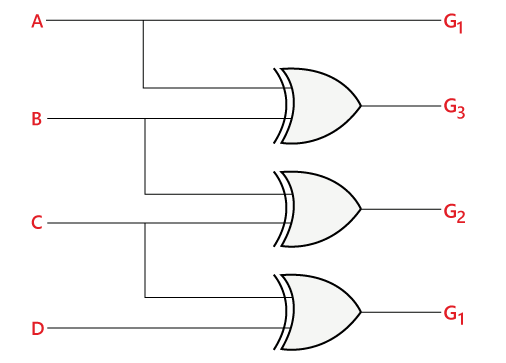
\includegraphics[scale=0.5]{binary_to_gray.png}
	\caption{Binary to Gray Code conversion using Logic Gates}
\end{figure}

\subsection{Gray to Binary Conversion Logic Gate Design}
\begin{figure}[H]
	\centering
	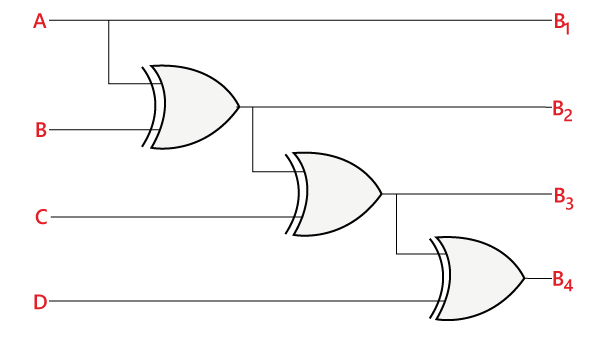
\includegraphics[scale=0.5]{gray_to_binary.png}
	\caption{Gray to Binary conversion using Logic Gates}
\end{figure}

\section{Circuit Diagrams}
\subsection{Pin Diagram of IC 7486}
\centering
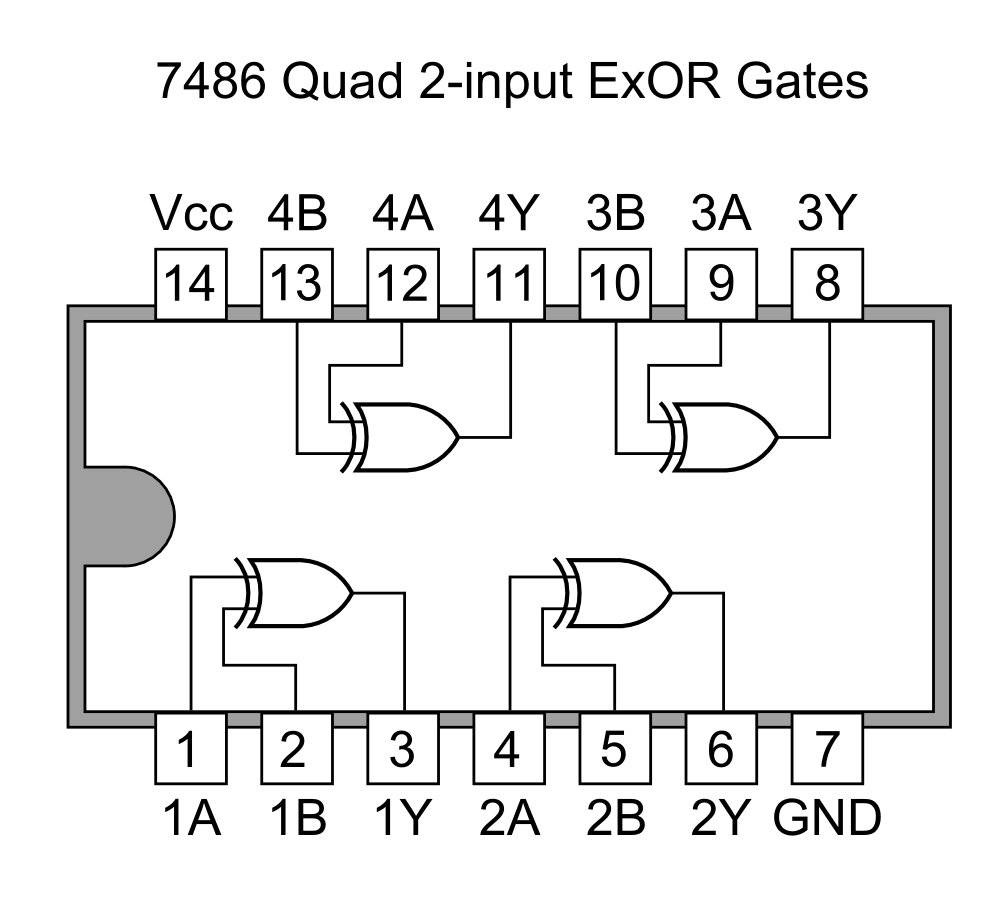
\includegraphics[scale = 0.3]{7486_Quad_2-input_ExOR_Gates.png}
\subsection{Circuit Diagrams for Conversions}
% 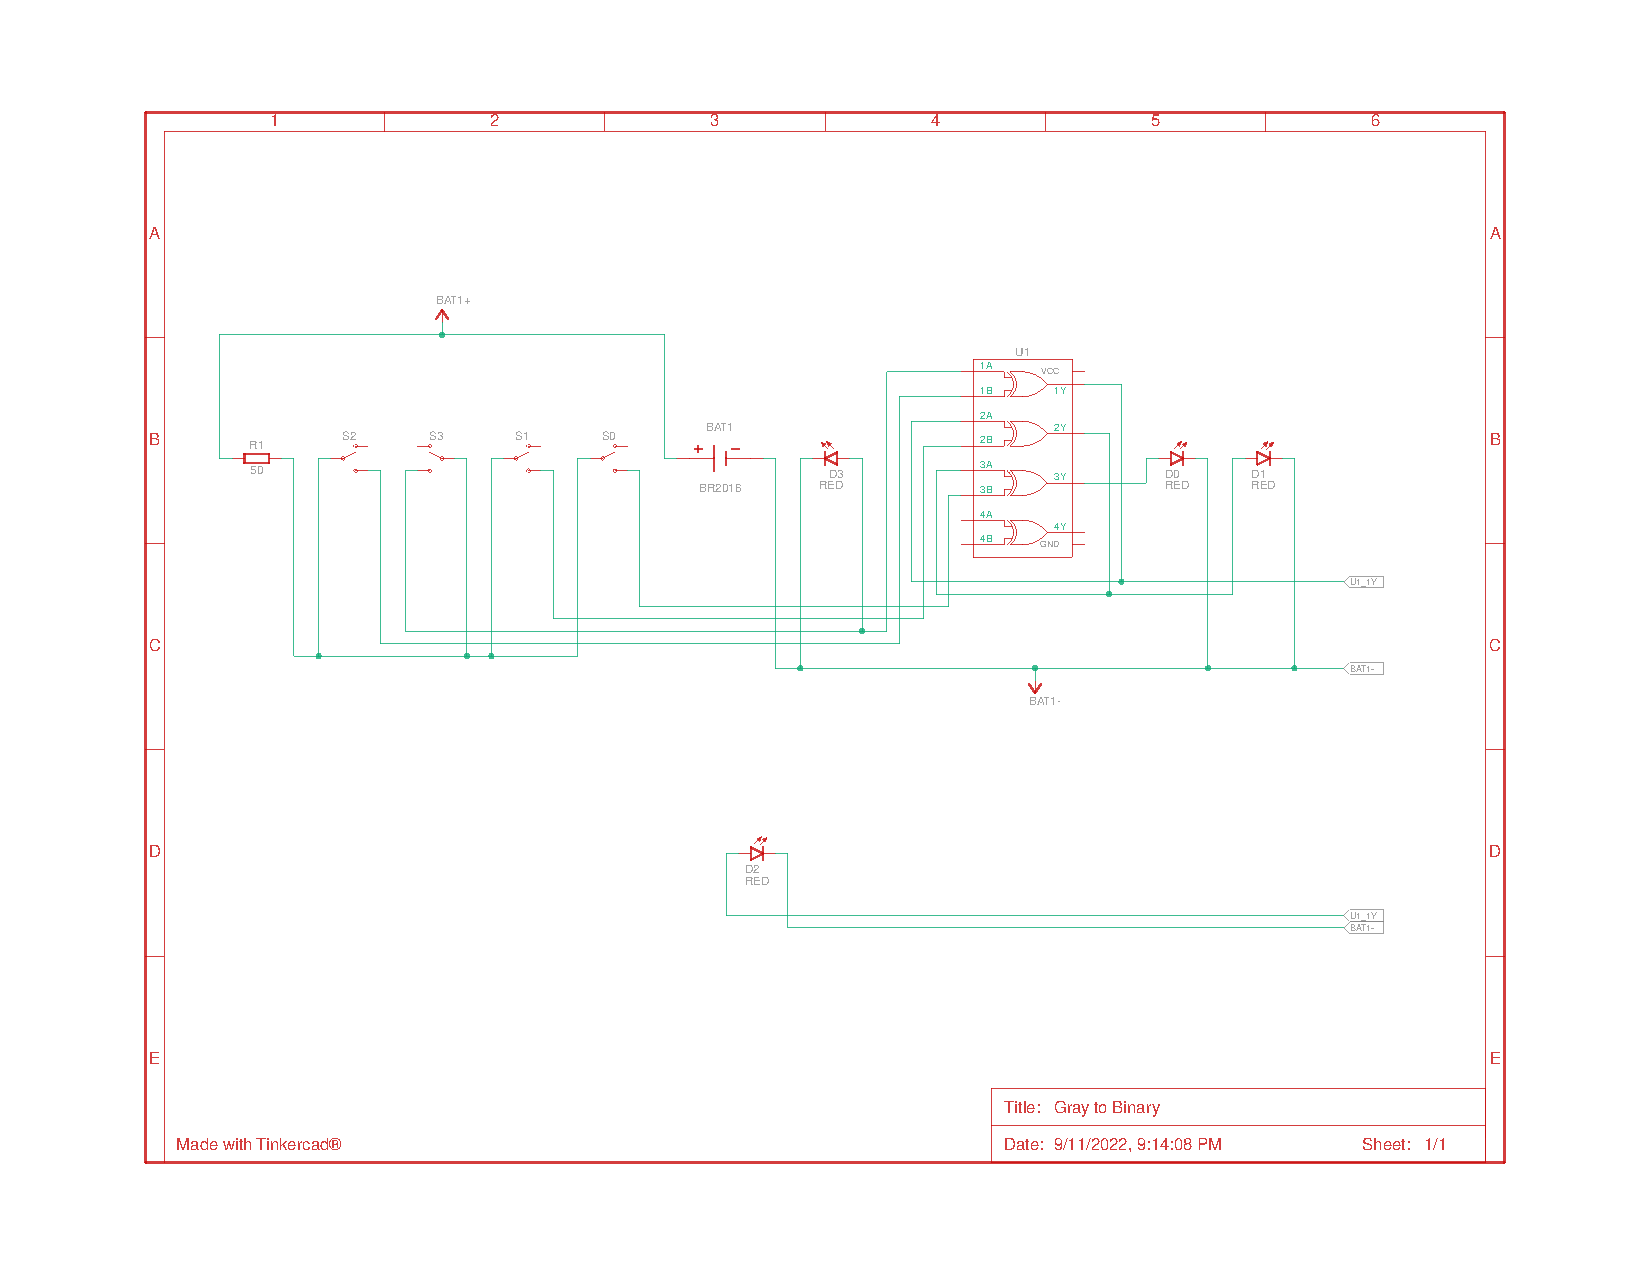
\includegraphics[scale = 0.5]{g_to_b.pdf}
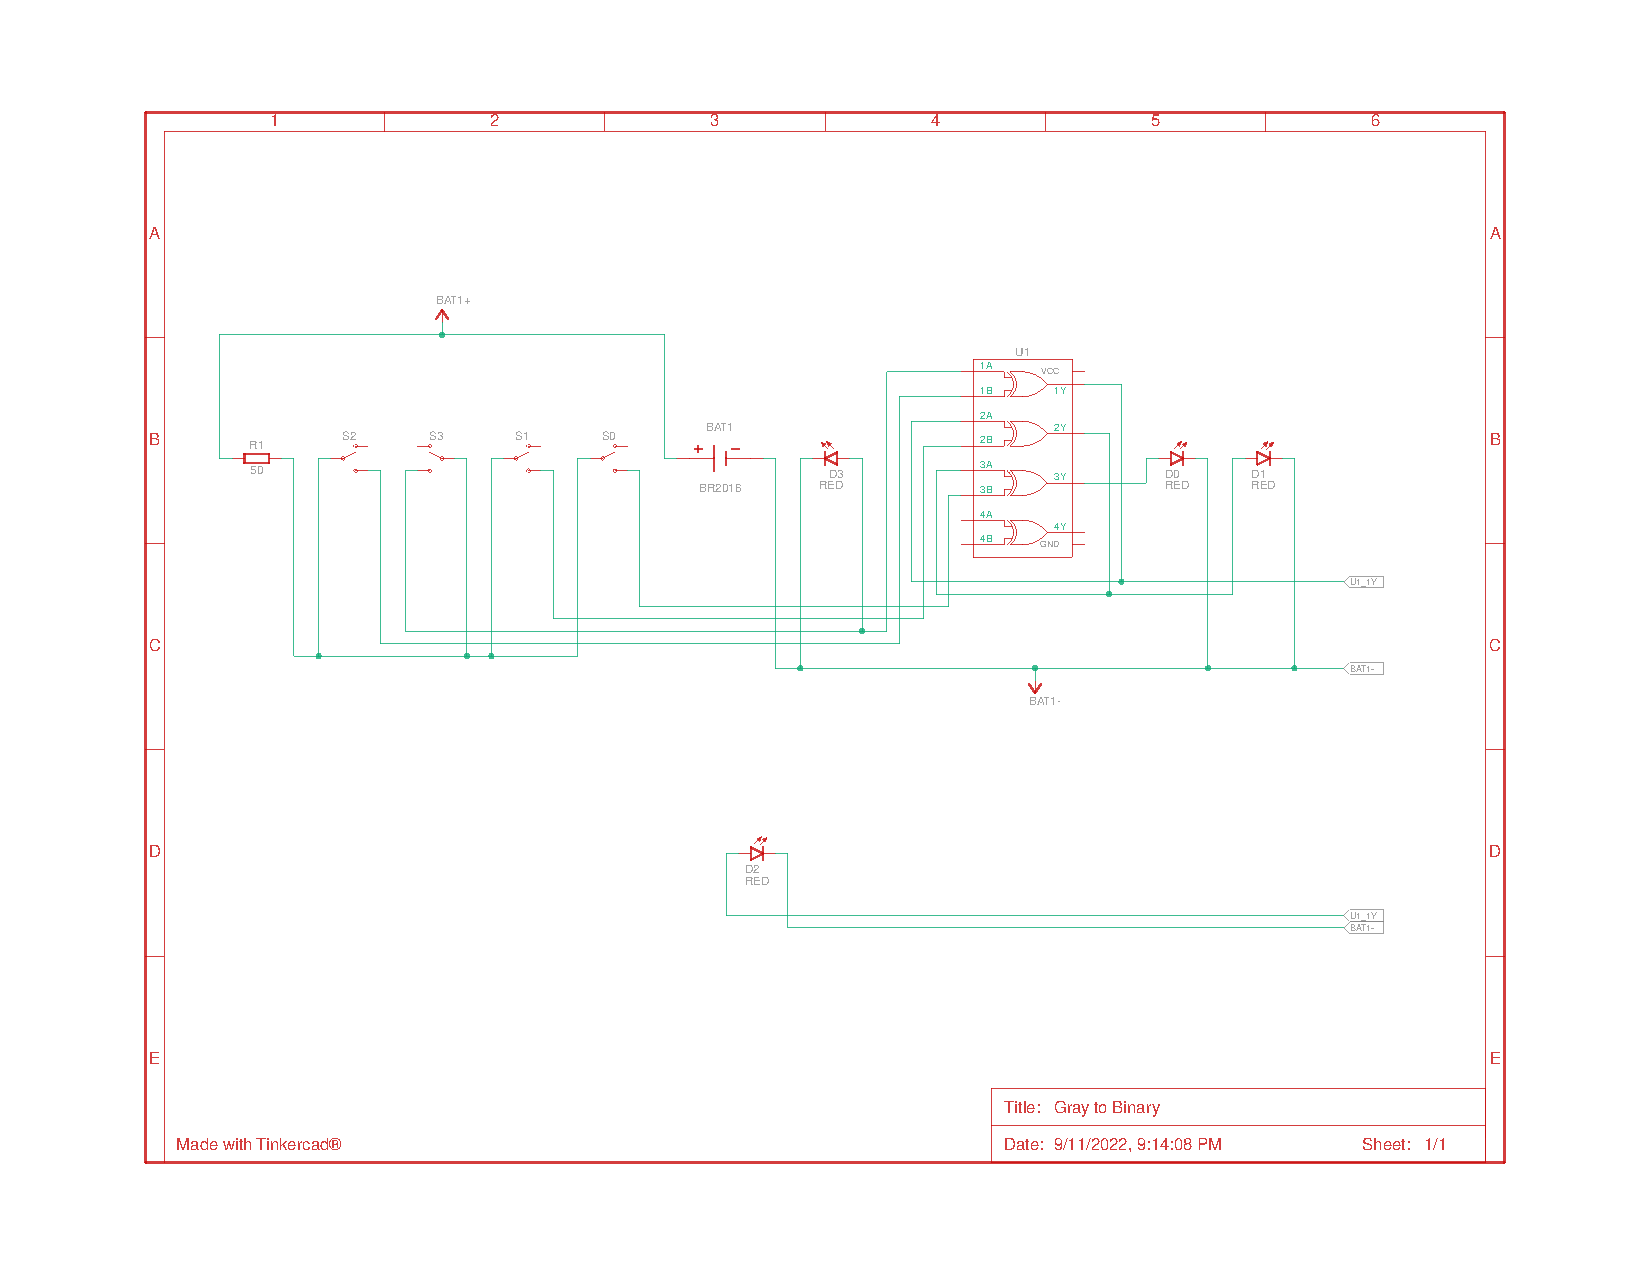
\includepdf{g_to_b.pdf}
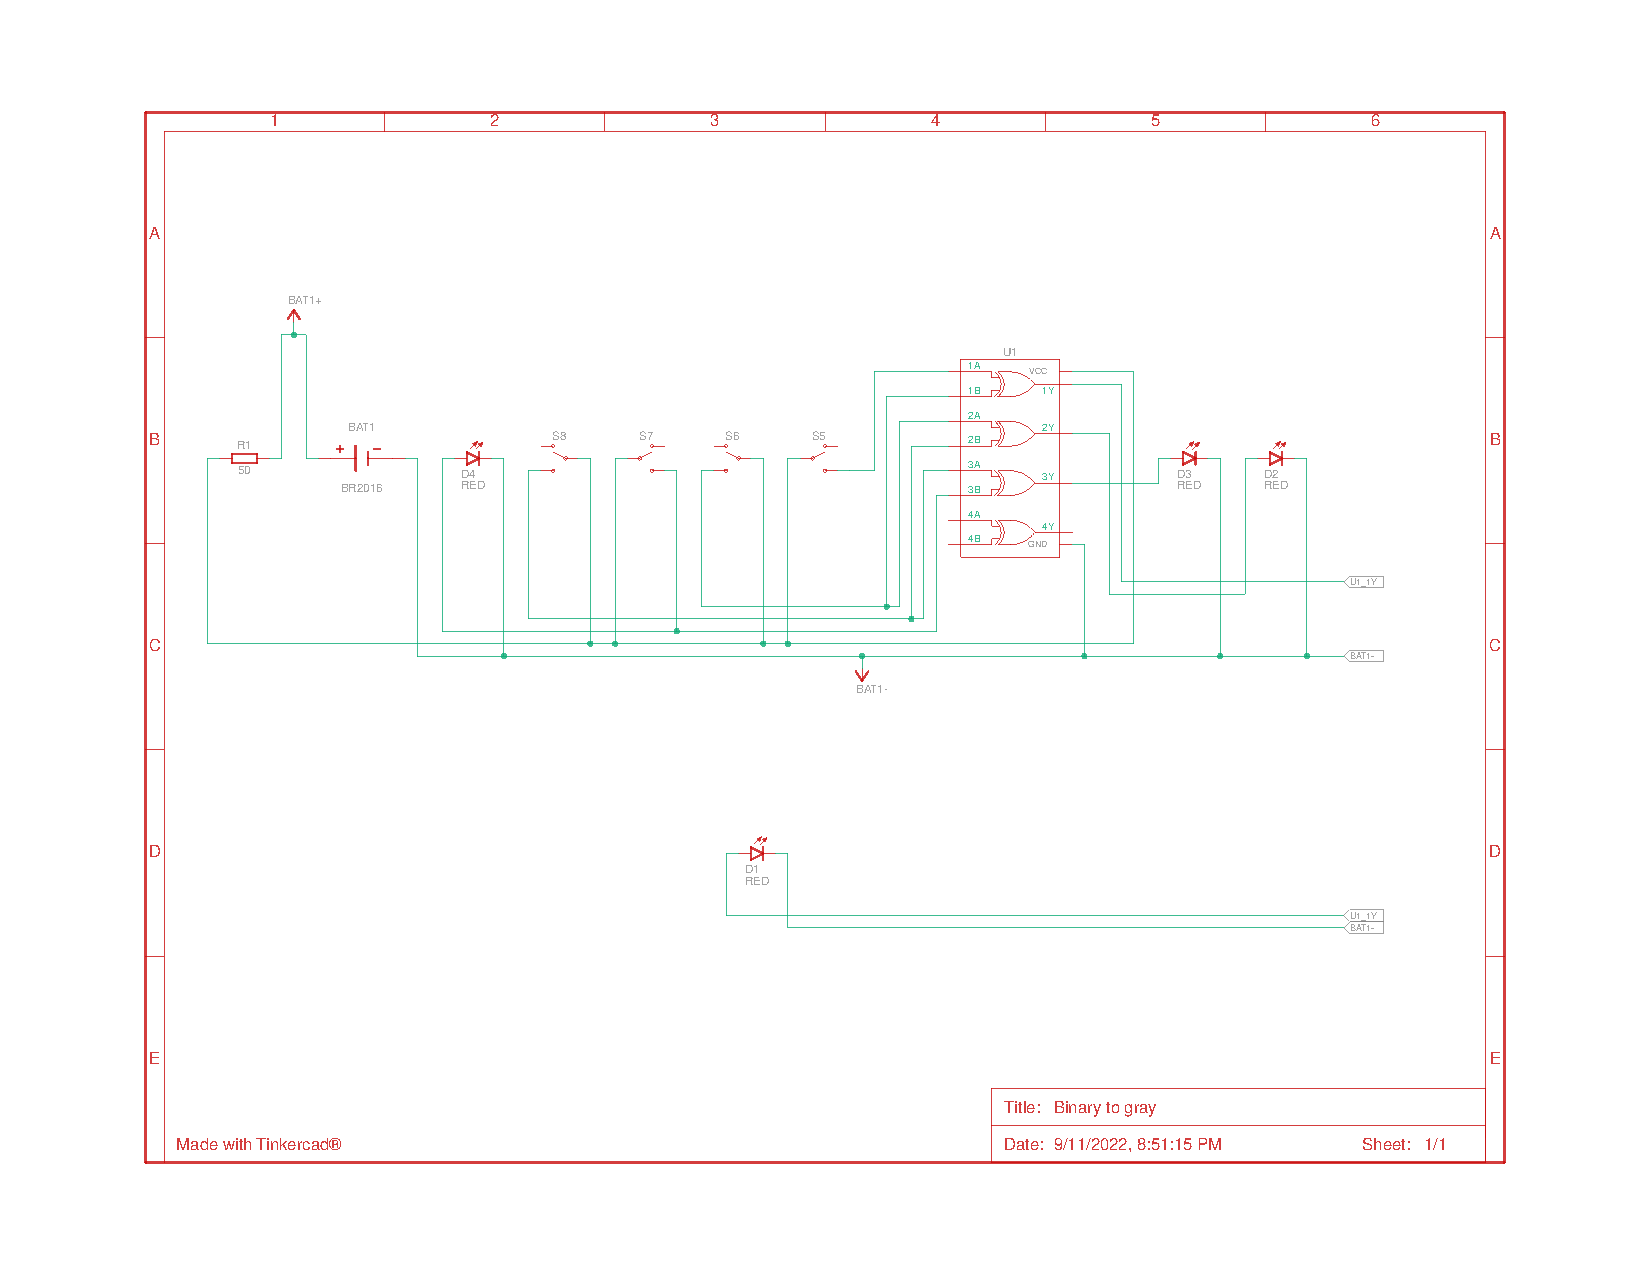
\includepdf{b_to_g.pdf}

\section{Procedure}

\begin{enumerate}
	\item Design Combinational logic circuits as per given problem statement.
	\item connect the IC 7486 and other basic logic gate ICs as per diagram.
	\item Give $V_{cc}$ supply and ground connection to each IC.
	\item Give variaous combinations to select lines.
	\item Observe the output and verify the truth table.
	\item Switch off the power supply off the trainer kit.
\end{enumerate}

\section{Conclusion}
We have learned the Implementation of Binary to Gray and Gray to Binary code converter using logic gates.


\section{FAQs}

\begin{enumerate}
	\item \textbf{Why is code conversion Necessary?}
	\begin{enumerate}
		\item Code conversions are most commonly used in computers, digital electronics, and microprocessors, etc. There are numerous codes like binary, octal, hexadecimal, Binary Coded Decimal (BCD), Excess-3, Gray code, Error Correcting Codes (ECCs) and ASCII code \dots
		\item Each Code just represents the basic numbers 1, 2, 3, 4, etc in a different Way. Each method is unique, and has some specific use. 
		\item In performing calculations and execution of certain algrithms, Certain types of codes may provide input that can be easily applied to the algorithm, as opposed to another type of code. 
		\item To Reduce the number of components used in a circuit, different types of such conversions from one code to another may be used, by applying different logic.
		\item An Example is Gray code, which is used in shaft encoders because The code of successive numbers differs exactly by one bit from its preceder.
		\item Excess- 3 is extensively used for subtraction because every code in XS-3 has its complement. 1s complement of the code yields 9s complement of a number itself.
		\item Alphanumeric codes by ASCII standards are widely used as a representation systems to the character set in computers.
		\item BCD is used in 7 Segment Displays
	\end{enumerate}
	
	\item \textbf{Write any 2 Applications of Gray Code}
	\begin{enumerate}
		\item The gray code is used in a few specific applications. The main applications include being used in analog to digital converters, as well as being used for error correction in digital communication. Gray code is used to minimize errors in converting analog signals to digital signals.
		\item Boolean circuit minimization
		\item Communication between clock domains
		\item Error correction
		\item Genetic algorithms
		\item Mathematical puzzles
		\item Position encoders
	\end{enumerate}
	\item \textbf{Explain Weighted and Non Weighted Codes with Examples}
	\begin{enumerate}
		\item Weighted Code: The weighted codes are those that obey the position weighting principle,which states that the position of each number represent a specific weight. 
		\item Example of a Weight Code would be Binary, BCD, hex, Octal, etc where each position has a certain weight.
		\item Non Weighted Codes: It is a type of code that does not have any positional weights associated with it. 
		\item Example would be Decimal, Binary, ASCII, Gray Code, etc. 
	\end{enumerate}
\end{enumerate}

\end{document}